Impulsu kodēšana ir būtiska \Gls{snn} sastāvdaļa, kas nosaka informācijas pārraides veidu ar diskrētiem impulsu laikiem. Dati jākodē impulsu virknēs, lai 3D punktu mākonis tiktu pārveidots laika informācijā \cite{safa2021}. Izmantota \Gls{tvc} metode, kas retinātus telpiski temporālus datus pārveido režģveida formātā nelielā laika soļu skaitā. Līdzīga pieeja atrodama darbos \cite{Cordone2022, fan2025}, kur to sauc par vokseļu kuba kodēšanu. Salīdzinājumā ar parasto vokseļu režģa kodēšanu \cite{bardow2016} vokseļu kuba kodēšana ļauj katrā laika solī kanālu dimensijā glabāt vairāk informācijas.

Veicot šo pārveidošanu, iegūst telpiskās informācijas vairāku soļu impulsu reprezentāciju. Šāda kodēšanas metode izmanto \Gls{snn} rekurento dabu.

Pirms pārveidošanas nepārtrauktā ģeometriskā punktu mākoņa reprezentācija vispirms tiek retināta, iegūstot jaunu diskrētu 3D režģa reprezentāciju, lai samazinātu turpmāko operāciju ieejas datu apjomu. Šādi samazinās atmiņas un skaitļošanas prasības bez būtiska informācijas zuduma, ja vokseļa izmērs ir izvēlēts pareizi. Ja dots sākotnējais nepārtrauktais punktu mākonis 3D telpā \(\mathcal{P} = \{(x_i, y_i, z_i) \mid x_i, y_i, z_i \in \mathbb{R}\}\) un vokseļa izmērs \([VS_x, VS_y, VS_z]\), vokseļu režģi var definēt kā šo punktu diskrētu attēlojumu 3D režģī \(\mathcal{V} = \{(x_v, y_v, z_v) \mid x_v, y_v, z_v \in \mathbb{Z}\}\). Pāreju no nepārtrauktās telpas uz vokseļu telpu attiecībā pret sākotnējā punktu mākoņa minimālajām koordinātām nosaka
\begin{equation}
  \begin{split}
    x_v = \floor*{\frac{x - x_{min}}{VS_x}},
    y_v = \floor*{\frac{y - y_{min}}{VS_y}},
    z_v = \floor*{\frac{z - z_{min}}{VS_z}}
  \end{split}
\label{eq:voxels}
\end{equation}
kur minimālās un maksimālās koordinātas ainā ir
$$[(x_{min}, y_{min}, z_{min}), (x_{max}, y_{max}, z_{max})].$$
Šīs ietverošā paralēlskaldņa vērtības nosaka vokseļu režģa telpiskās robežas un ietekmē vokselizētās reprezentācijas izšķirtspēju. Tā kā vokseļa izmērs īpaši būtiski ietekmē XY plaknes izšķirtspēju, ietverošā paralēlskaldņa apjoms pēc iespējas tiek samazināts, lai līdzsvarotu aprēķinu efektivitāti un telpisko precizitāti. Ar šo metodi tīkls var novērtēt nelielu skaitu \(C \times H \times W\) formas \Gls{bev} pseidoattēlu. Iegūto diskrēto laika soļu skaits ir
\begin{equation}
  T = \frac{z_{max} - z_{min}}{VS_z}.
  \label{eq:T}
\end{equation}

Vokselizācijas process tiek paplašināts ar papildu kvantēšanu, sīkāk sadalot \(T\) laika soļus laika intervālos. Tas ietver z dimensijas sadalīšanu \(n\) diskrētos intervālos:
\begin{equation}
    t_{bin} = \floor*{\frac{(z - z_{min})\ \mathrm{mod}\ VS_z}{Q}},
    \label{eq:bins}
\end{equation}
kur \(Q = VS_z/n\) ir intervāla izmērs. Lieki aprēķini tiek papildus novērsti, apvienojot operācijas vienādojumos (\ref{eq:voxels}) un (\ref{eq:bins}). Šī modifikācija ļauj iegūt detalizētāku informāciju z dimensijā, pielāgojot detalizācijas pakāpi. Ar šo reprezentāciju izveido 4D tenzoru ar formu \(T \times C \times H \times W\), kur \(H\) un \(W\) ir datu augstums un platums, \(C\) ir kanālu skaits katrā laika solī un \(T\) ir laika soļu skaits. Sīkāk sadalot vokseļus un glabājot papildu informāciju kanālu dimensijā, vokseļu intervāli ļauj palielināt izšķirtspēju, nepalielinot laika soļu skaitu.

Ja LiDAR vietā izmanto \Gls{tof} datus, kā parādīts \ref{fig:3dscnn_tof_arch}. attēlā, datus iegūst no vairākiem izkliedētiem sensoriem. Pirms temporālās vokselizācijas atsevišķie punktu mākoņi jāpārveido kopīgā koordinātu sistēmā. Katram sensoram stingro transformāciju aprēķina no blakus esošo sensoru pārklāšanās apgabala. Reģistrācijas procedūrā punktu mākoņu transformāciju pārus novērtē, identificējot atbilstošas ģeometriskās pazīmes. Šajā darbā tam izmanto \Gls{dgr}, ievērojot uz pazīmēm balstītu punktu mākoņu reģistrācijas pieeju, kas aprakstīta darbos \cite{choy2020, choy2019a, choy2019b, li2021}. Transformācijas piemēro atsevišķajiem punktu mākoņiem, iegūstot vides reprezentāciju kopīgā koordinātu sistēmā.

\begin{figure}[ht]
    \centering
    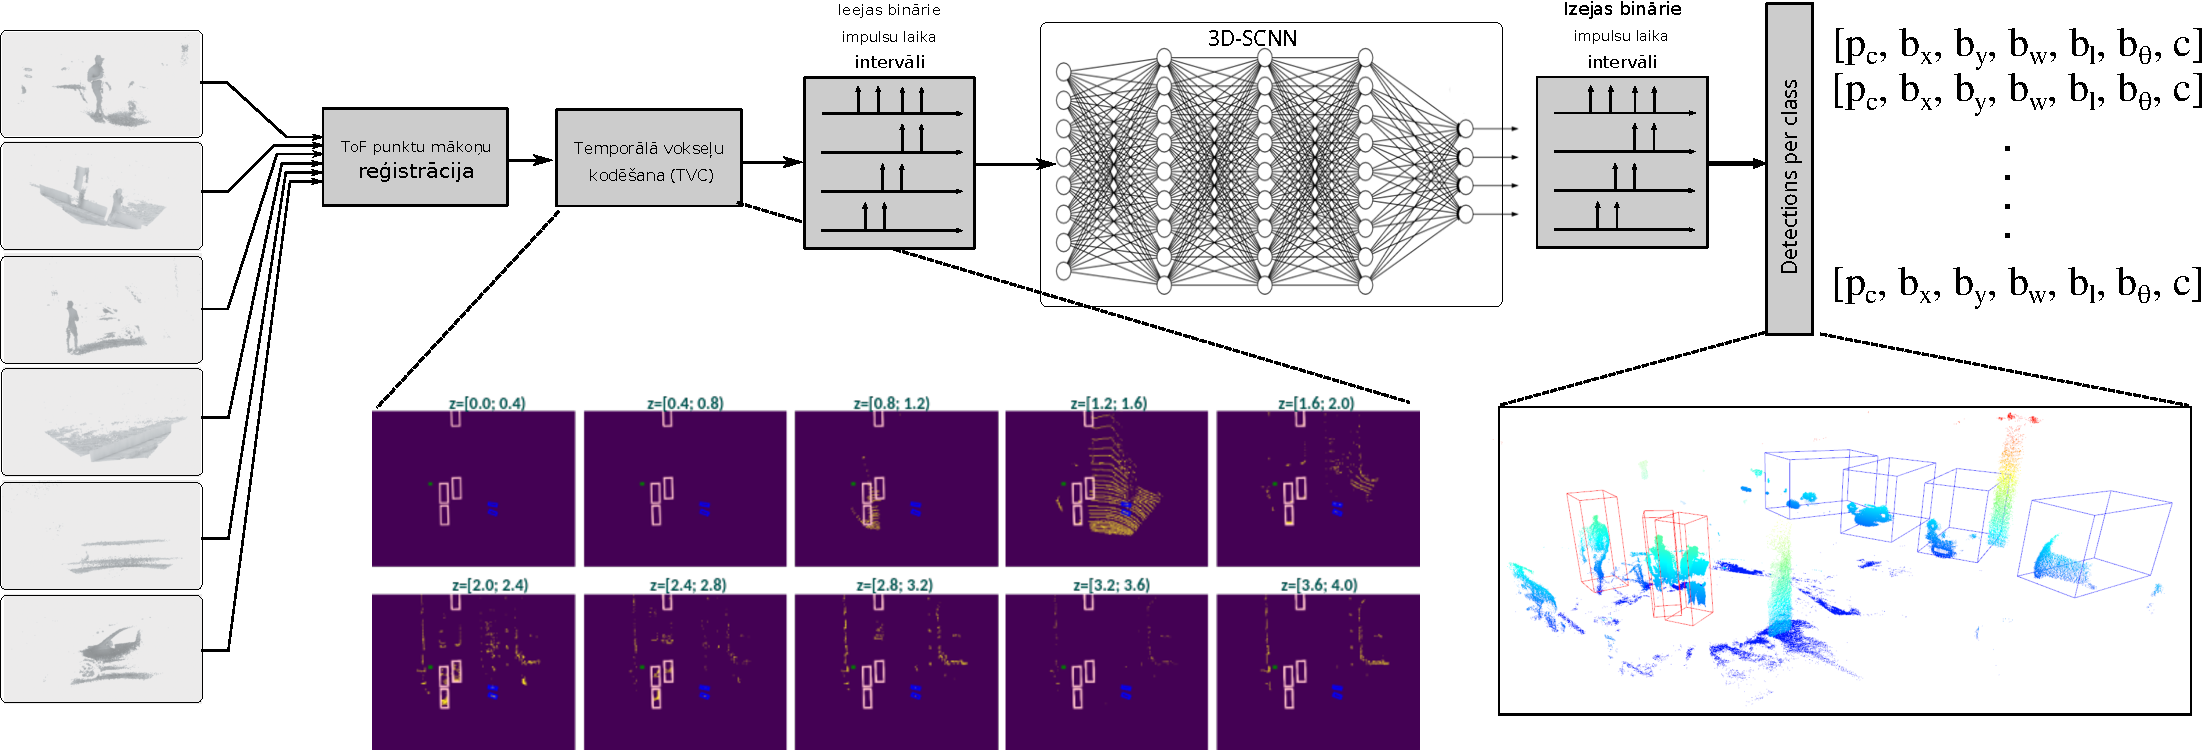
\includegraphics[width=\textwidth]{fig/lv/3dscnn_architecture-v3.pdf}
    \caption{3D-CSNN arhitektūra. Vairāku ToF sensoru nepārtrauktā punktu mākoņu telpa tiek reģistrēta un retināta, izveidojot diskrētus režģus vairākos laika soļos objektu detektēšanai ar 3D konvolucionālu \Gls{snn}.}
    \label{fig:3dscnn_tof_arch}
\end{figure}


